%%%%%%%%%%%%%%%%%%%%%%%%%%%%%%%%%%%%%%%%%%%%%%%%%%%%%%%%%%%%%%%%%%%%%%%%%%%%%%%%%%%%%%%%%%%%%%%%%%%%%%
%
%   Filename    : chapter_1.tex 
%
%   Description : This file will contain your Research Description.
%                 
%%%%%%%%%%%%%%%%%%%%%%%%%%%%%%%%%%%%%%%%%%%%%%%%%%%%%%%%%%%%%%%%%%%%%%%%%%%%%%%%%%%%%%%%%%%%%%%%%%%%%%

\chapter{Research Description}
\label{sec:researchdesc}    %--note: labels help you with hyperlink editing (using your IDE)

This chapter is an overview of the research on community detection in social networks. 
The current state of the technology, objectives, scope, limitations, and significance of the research is 
included here.

\section{Overview of the Current State of Technology}
\label{sec:overview}

Social media has become much more prevalent in recent years. People can now participate in what is called microblogging, a way for people to share their thoughts, status, and opinions in short posts, like Twitter, where posts are limited to one-hundred and forty characters. \cite{Java:2007}. As such, these social media platforms are a prime opportunity to mine sentiments and to detect communities in the social network. 

Numerous studies on community detection have already been done. \citeA{Zhang:2012} defined features that can be used to identify similarity and aggregated these similarities to detect communities. \citeA{Lim:2012:1} performed an inverted version in which they first defined interests and based on these interests, sought to extract communities from the network. Individual opinions of one specific user towards another was also studied by combining sentiment analysis with network analysis \cite{West:2014}. Some visualizations have already been created such as SocialHelix by \citeA{Cao:2015} which depicts two sides of an argument as strands in a helix and their intersection defines events.

However, it is noticeable that most of these studies mostly involved Twitter. As far as our research goes, there has yet to be a community detection tool that integrates Facebook, as well as Twitter, into the computation. In this research, we aim to address the fact that such a system does not yet exist by developing a visualization tool for community detection using sentiment analysis on the social networks Facebook and Twitter.

\begin{comment}
This section gives the reader an overview of the specific technology or field in the international or
local setting. The information regarding the technology or field should be contemporary and not
based on outdated sources. Discussion must not be too technical or too detailed.

\textcolor{red}{This section ends with a discussion on the problem/s faced by or that still exist in the specific
technology or field (e.g., limitations of existing software or algorithms). The problem statement
would lead to the research objectives.}


It is   easy to include a figure in JPG or PNG format as shown in the 
following example.  Make sure that you explain what the figure is all about,
and that you refer to your figure.  For example, \figref{fig:disneystock} shows a graph of the performance of Disney stock from the 1980s to 2012.

%--- the following example shows how to include a figure in PNG format
\begin{figure}[t]                %-- use [t] to place figure at top, [b] to place at the bottom, [h] for here
\centering                    %-- use this to center the figure
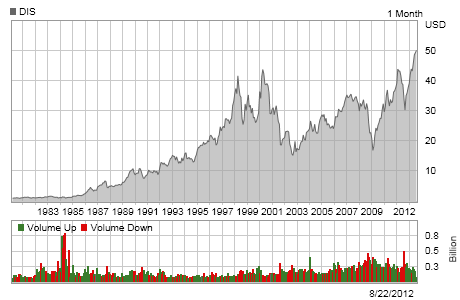
\includegraphics{DisneyChart.png}      %-- include image file named as "disneychart.png" 
\caption{This is the figure's caption -- Disney stock chart}
\label{fig:disneystock}
\end{figure}


Some notes on citing references.   When using APA format, the author-date method of citation is 
followed.   This means that the author's last name and the year of publication for the source should 
appear in the text, and a complete reference should appear in the reference list.

%
% Examples:
%     	Smith (1970) compared reaction times . . .
%     	In a recent study of reaction times (Smith, 1970), . . .   
%     	In 1970, Smith compared reaction times . . .
%	Smith, et al., (1970) compared reaction times . . .
%     	In a recent study of reaction times (Smith, et al., 1970), . . .  
%     	In 1970, Smith, et al., compared reaction times . . .
%

Here are some examples on how to do the referencing (note author's name and years are different
from commented examples).  For APA citation details, refer
to \url{http://www.ctan.org/tex-archive/biblio/bibtex/contrib/apacite/}. 

\begin{itemize}
\item \citeA{Amor:2015} compared reaction times...
\item In a recent study of reaction times \cite{Bakillah:2014}...
\item In \citeyearNP{Bryden:2013}, \citeauthor{Cao:2015} compared reaction times...
\item \shortciteA{Clauset:2004} compared reaction times... 
\item In a recent study of reaction times \cite{Darmon:2015}...
\item In \citeyearNP{Deitrick:2013}, \shortciteauthor{Java:2007}, compared reaction times...
\end{itemize}

The following are references from journal articles \cite{Lancichinetti:2011}.  Here's an MS thesis document \cite{Lim:2012:0}, and this is from
PhD dissertation \cite{Lim:2012:1}. For a book, reference is given as 
\cite{Papadopoulos:2012}.  Proceedings from a conference samples are \cite{Pearce:2014}.  The sample bibliography file named \textbf{myreferences.bib} is from the
SIGGRAPH \LaTeX template.  You can use a text editor to view the contents of the bib file.  
It is your task to create your own bibliography file.  For those who downloaded papers from
ACM or IEEE sites, there is a BibTeX link that you can click; thereafter, you just simply need
to copy and paste the BibTeX entry into your own bibliography file.



The following shows how to include a program source code (or algorithm).  The verbatim environment,\cite{West:2014,Xie:2012,Zhang:2012}
as the name suggests, outputs text (including white spaces) as is...

\begin{verbatim}
#include <stdio.h>
main()
{
printf("Hello world!\n");
}
\end{verbatim}


\textcolor{red}{DO NOT FORGET to write the statement of the research problem here, i.e.,
before the Research Objectives.}
\end{comment}


\section{Research Objectives}
\label{sec:researchobjectives}

\subsection{General Objective}
\label{sec:generalobjective}

This research's end goal is to produce a visualization of the detected communities.


\subsection{Specific Objectives}
\label{sec:specificobjectives}

\begin{enumerate}
	\item To determine the various techniques and algorithms in detecting communities;
	\item To determine the appropriate parameters to use in detecting the communities;
	\item To determine how to evaluate the correctness of the detected communities
\end{enumerate}

\section{Scope and Limitations of the Research}
\label{sec:scopelimitations}

In detecting communities, our research will be limited to algorithms we found in our review of related literature, including the Infomap algorithm, speaker-listener label propagation algorithm, Markov stability, clique percolation method, k-means clustering, and divisive hierarchical clustering.

In identifying parameters, our research is limited to sentiment analysis and elements which can be extracted from a user’s post, which may include follow networks, hashtags, mentions, and retweets, which were mostly inspired from literature which focused on Twitter \cite{Deitrick:2013,Zhang:2012,Lim:2012:1}. As such, Facebook specific features such as membership in groups and event participation may also be considered.

In community evaluation, only average mutual following links per user per community or FPUPC \cite{Zhang:2012}, modularity \cite{Deitrick:2013},  and clustering coefficient \cite{Lim:2012:1} will be considered in evaluating communities.

\section{Significance of the Research}
\label{sec:significance}

This section explains why research must be done in this area.  It rationalizes the objective of the research with that of the stated problem. 
Avoid including sentences such as ``This research will be beneficial to the proponent/department/college'' as this is already an inherent
requirement of all BS and MS thesis projects.  Focus on the research's contribution to the Computer Science field.

The following are guide questions that may help your formulate the significance of your research. 


%
% IPR acknowledgement: the following list of items are from Ethel Ong's slides on Significance of the Research
%
\begin{itemize}
	\item  What is the relevance of your work to the computer science community? 
	
	\begin{itemize} 
		\item What will be your technical contributions, in terms of algorithms, or approaches, or new domain? 
		\item What is your value-added compared to existing systems? 
	\end{itemize}
	
	\item What will be your contributions to society in general? 
	\begin{itemize}
		\item This research will help certain stakeholders understand the common sentiments from social media users.
		\item This research will be useful in finding points of improvement in relevant institutions.
	\end{itemize}
\end{itemize}

This research will help certain stakeholders understand the common sentiments from social media users. Analysis of social media networks can give better insight into the workings of real world society \cite{Papadopoulos:2012}. 



